% !TEX root = BA-Bauer.tex
\newpage
\section{Zusammenfassung}
In der vorangegangen Praxisprojektarbeit wurden Grundlagen erarbeitet, welche die Aufnahme und Wiedergabe von DMX-Datenströmen mit einem Mikrocontroller ermöglichen. Die entwickelte Hard- und Software eigneten sich nicht für eine nützliche Anwendung in der Praxis.\\
Ziel dieser Arbeit ist die Implementierung und Weiterentwicklung der erarbeiteten Grundlagen der Praxisprojektarbeit in einen Prototypen eines Produktes mit gewisser Marktreife.\\
Zum Erreichen dieses Ziels wird eine Benutzerschnittstelle entwickelt, die eine Bedienung des Gerätes ermöglicht. Dazu gehört die Auswahl von Hardwarekomponenten, die Entwicklung einer elektrischen Schaltung und entsprechender Software. Zudem wird eine Platine entworfen, welche in einem passenden Gehäuse montiert wird.\\
Das Ergebnis dieser Arbeit ist ein funktionsfähiger Prototyp mit einer deutlich erkennbaren Marktreife, zu sehen in den nachstehenden Abbildungen.
\begin{figure}[h]
	\begin{minipage}{.45\linewidth}
		\centering
		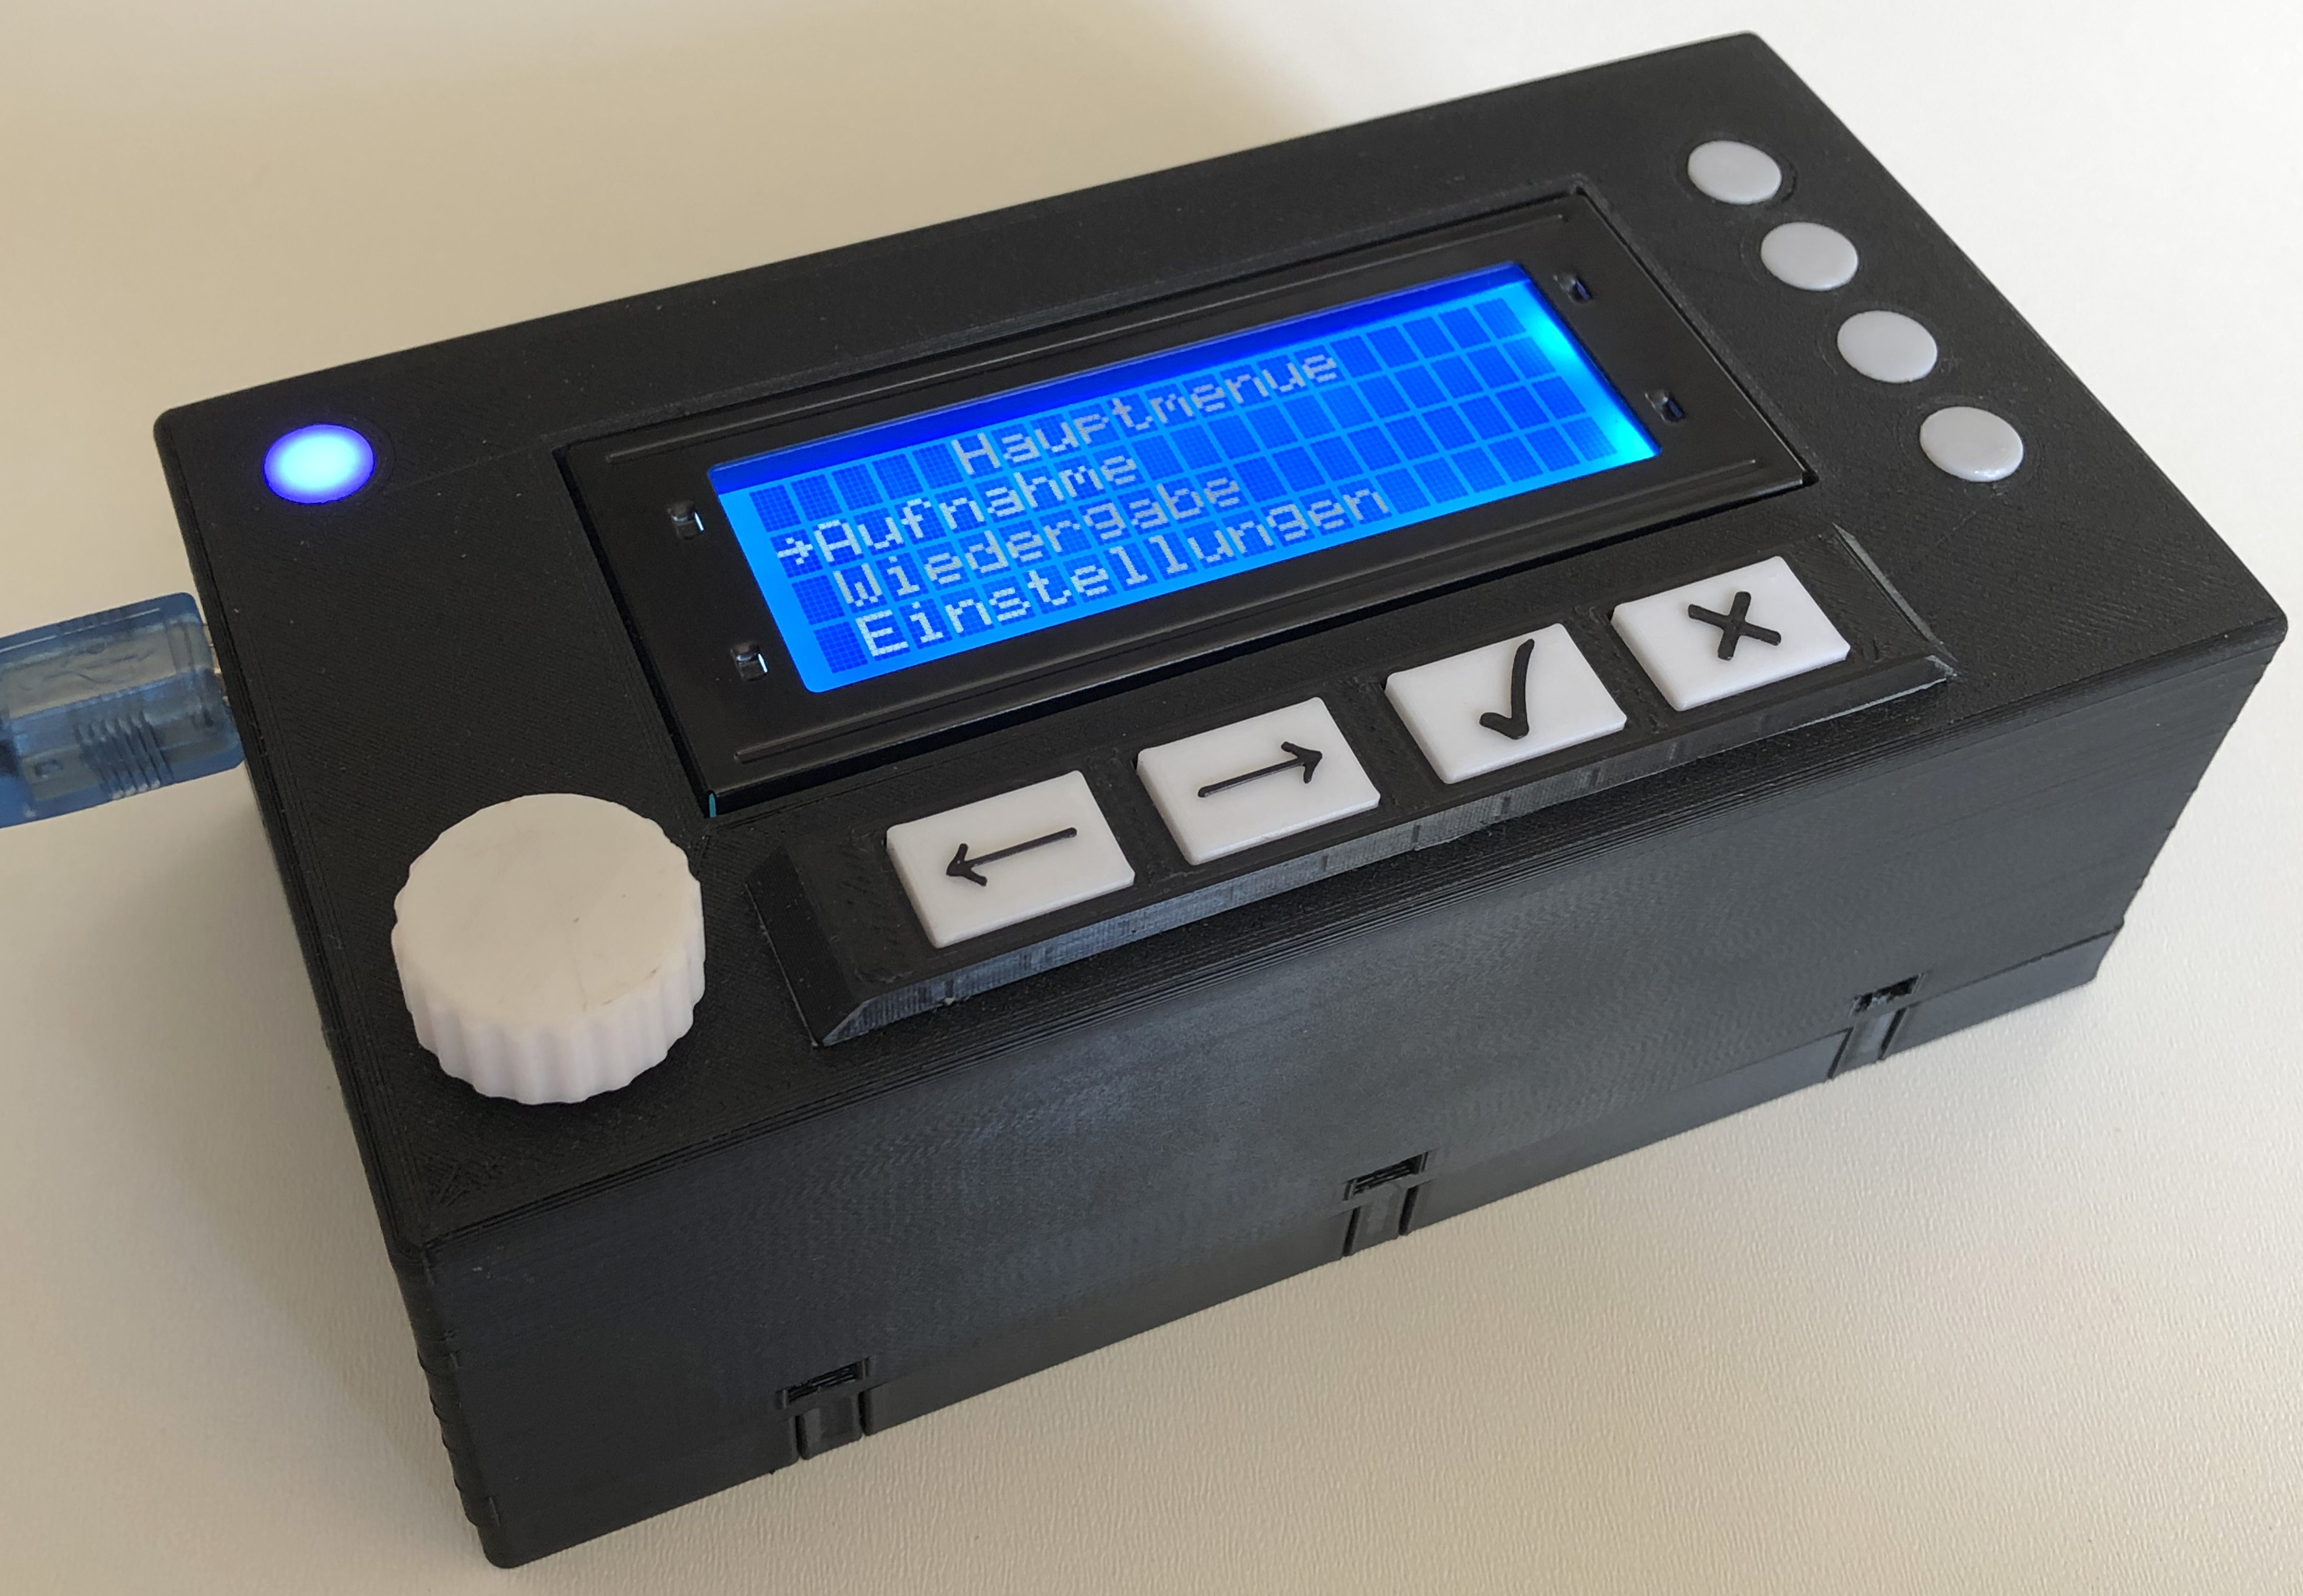
\includegraphics[width=\linewidth]{Resultat/Vorderseite}
		\caption{DMX Aufnahme und Wiedergabegerät - Vorderseite}
	\end{minipage}
	\hfill
	\begin{minipage}{.45\linewidth}
		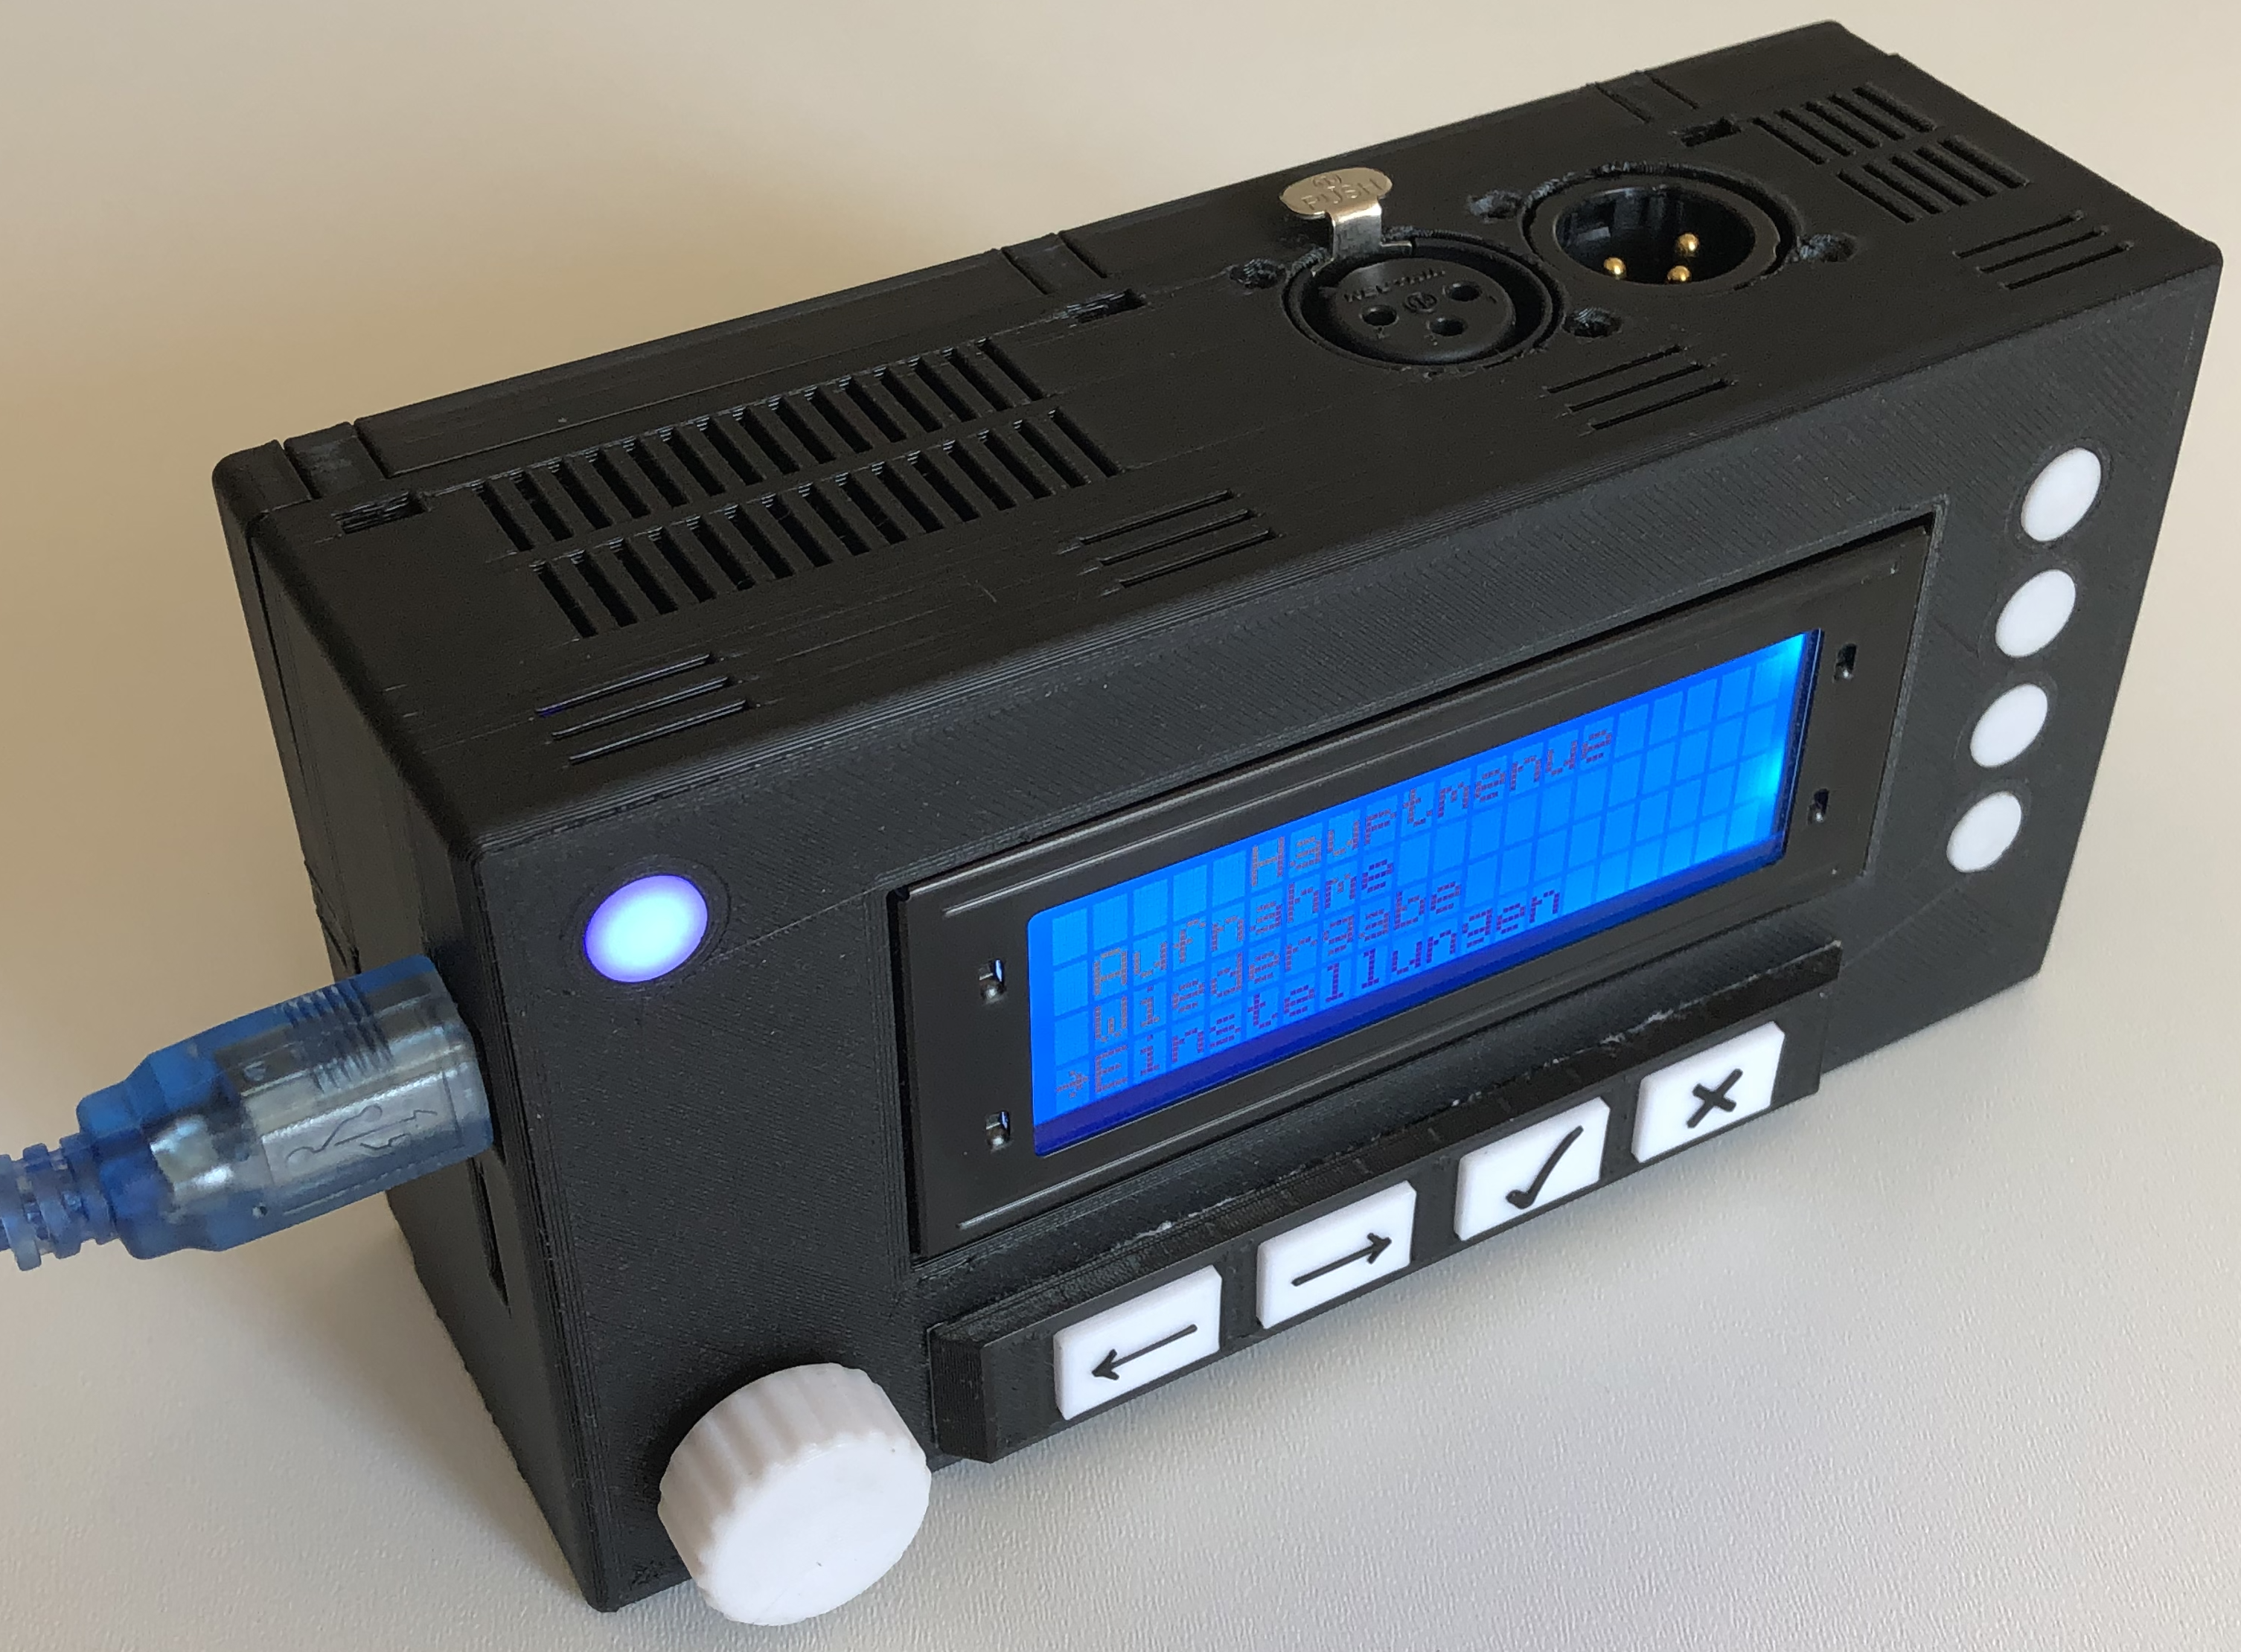
\includegraphics[width=\linewidth]{Resultat/Aufgestellt}
		\caption{DMX Aufnahme und Wiedergabegerät - Rückseite}
	\end{minipage}
\end{figure}
Die Weiterentwicklung und Erweiterung der Grundlagen aus der Praxisprojektarbeit ermöglichen dem Benutzer die Aufnahme und Wiedergabe von DMX-Daten in verschiedenen Modi. Eine variabel einstellbare Aufnahmezeit und die Möglichkeit, mehrere Aufnahmen anzulegen, stellen eine deutlich praxisnähere Verwendbarkeit her. Eine Erkennung von Übertragungsfehlern während der Aufnahme lässt eine zuverlässige Aufnahme zu. Die Implementierung einer umfassenden Benutzerschnittstelle, bestehend aus einem Display, Tastern, LEDs und einem Drehgeber, ermöglicht intuitive Eingaben des Benutzers und Rückmeldungen an den Benutzer. Nützliche Fehlermeldungen erleichtern die Behebung von eventuell auftretenden Fehlern. Statusanzeigen in Form von aufblinkenden LEDs in verschiedenen Farben lassen die Überprüfung der Funktion des Gerätes auf größere Entfernung zu. Ein Menü mit einfacher Menüführung hilft dem Benutzer alle Funktionen des Geräts intuitiv und ohne spezielle Vorkenntnisse zu verwenden. Über die Einstellungsmöglichkeiten kann der Benutzer die Funktion des Gerätes und die Optik der Benutzerschnittstelle auf die persönlichen Bedürfnisse anpassen. Ein Gehäuse in einer handlichen Größe lässt eine Vielzahl an Einsatzgebieten zu. Die zu Beginn der Arbeit definierten Hauptanforderungen sind vollständig erfüllt.\\%Nebenanforderungen?
Die in der Praxisprojektabeit erarbeiteten Grundlagen sind erfolgreich in einen Prototypen mit erkennbarer Marktreife implementiert und bieten das Potential einer Weiterentwicklung bis zum Erreichen der tatsächlichen Marktreife. 
